\chapter{Einleitung}
% \marktodo{Lieber Korrekturlesende! Zur Erklärung: Die roten Schriften sind Notizen an mich selbst von todos etc., nicht wundern.} 

% Hier folgt eine kurze Einleitung in die Thematik der Bachelorarbeit.
% Die Einleitung muss kurz sein, damit die vorgegebene Gesamtlänge der 
% Arbeit von 25 Seiten nicht überschritten wird. 
% Die Beschränkung der Seitenzahl sollte man ernst nehmen,
% da Überschreitung zu Abzügen in der Note führen kann. 
% Um der Längenbeschränkung zu genügen, darf auch nicht an der Schriftgröße,
% dem Zeilenabstand oder dem Satzspiegel (bedruckte Fläche der Seite) manipuliert werden.

Das Ruhrgebiet ist aus historischer Sicht für den Bergbau bekannt.
% Heutzutage gibt es im Ruhrgebiet keinen aktiven- oder Steinkohleabbau
% mehr\footnote{Das letzte Steinkohlebergwerk Prosper-Haniel Bottrop schloss am.
% 21. Dezember 2018.}.
Heutzutage gibt es im Ruhrgebiet allerdings keinen aktiven Braun- oder Steinkohleabbau
mehr\footnote{Das letzte Steinkohlebergwerk Prosper-Haniel Bottrop schloss am.
21. Dezember 2018.}.

Beim Bau und während der Benutzung musste rund um die Uhr mit Pumpen dafür gesorgt werden,
dass die Stollen nicht überfluten. Jene Bodenschichten besitzen von Natur aus ein 
gewisses Hohlraumvolumen, welches naturgemäß mit Wasser gefüllt ist.

Trotz sukzessiver Stilllegung der Bergwerke in den letzten Jahrzehnten
muss allerdings weiterhin der Wasserstand der Stollen mit Pumpen unter Kontrolle gehalten werden.
Dies geschieht aus zwei Gründen: \\
Zum einen ist durch den massiven Bergbau im Ruhrgebiet im Laufe des letzten Jahrhunderts 
das Ruhrgebiet allmählich abgesackt und unter den Grundwasserspiegel gesunken. 
Ein Vernachlässigen der Wasserstände hätte zur Konsequenz, dass ganze Städte überflutet würden 
(siehe Abb. \ref{fig:Ruhrgebiet_Seen}). Zum anderen sind Verschmutzungen des Grubenwassers
\footnote{Verschmutzungen Steinkohlenbergwerke z.B.: Nickelsulfat, Eisenoxide und Mangan.\cite{grubenwasser}}
\footnote{Verschmutzungen Braunkohlenbergwerke z.B.: Kalzium, Eisenmonoxid, Zink, Magnesium,
 Natrium, Ammonium und Mangan \cite{grubenwasser}}.
Es soll verhindert werden, dass das Grubenwasser unser Grundwasser
und somit teilweise auch das Trinkwasser verschmutzt.


Die Forschungsfrage dieser Arbeit ist es herauszufinden, inwiefern mithilfe der Myographie 
der Wasserstand in einem stillgelegten Bergbaustollen gemessen werden kann. 

Es wird die Zählrate eines Detektors am Boden einer Bohrung simuliert.
Aus den Informationen der Bohrung wird als Fundament für die Simulation 
ein Bodenmodell erstellt.
Es werden verschiedene Wasserhöhen aus den für den Bergbau drainierten Bodenschichten modelliert.
Es wird untersucht, wie sensitiv die Zählrate des Detektors auf veränderliche Wasserstände ist. 
\\
Der Myonenfluss wird mit EcoMug bestimmt und die Myonen mit PROPOSAL simuliert.

\begin{figure}[]
   \centering
   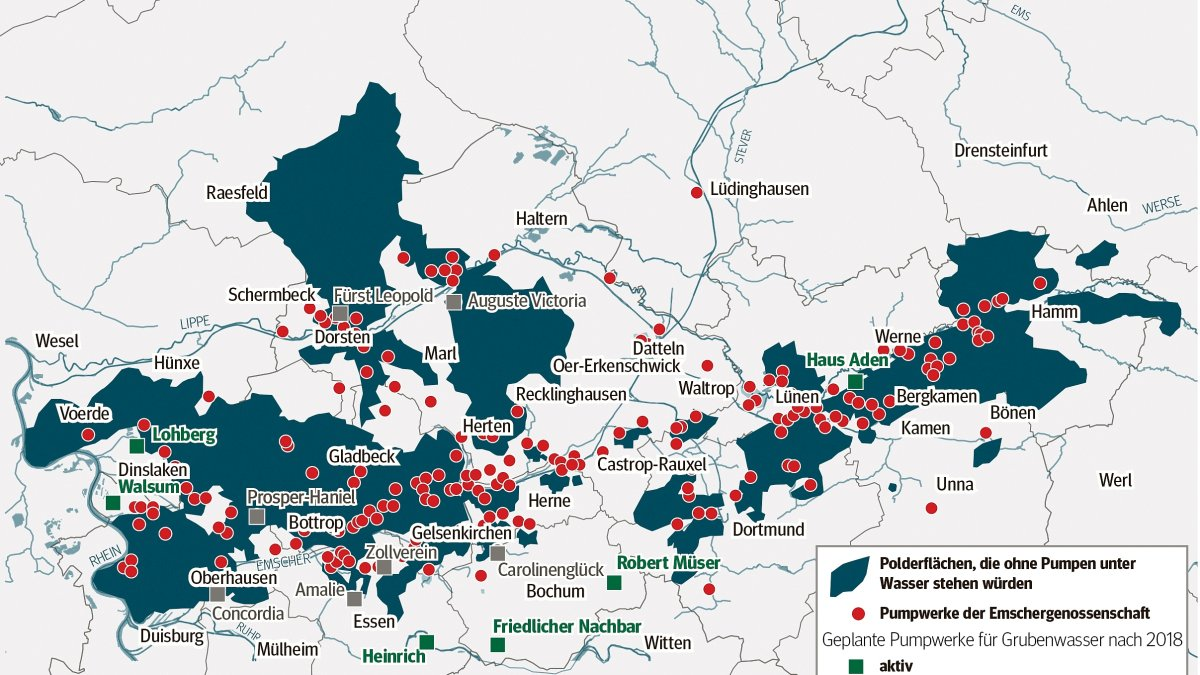
\includegraphics[width=\textwidth]{ruhrgebiet_unter_wasser.jpg}
   \caption{In Dunkelblau die Regionen im Ruhrgebiet, welche aufgrund der Absenkungen 
   unter Wasser stehen würden, wenn nicht ständig gepumpt werden würde. 
   2019 betrugen sich die Kosten für die Pumpwerke auf 220 Millionen Euro\cite{waz_seen}}
   \label{fig:Ruhrgebiet_Seen}
\end{figure}

% Zum Schluss wir die Simulation auf einen Detektor übertragen und 
% Messzeiten für eine Detektor ausgerechnet.

%  \marktodo{
%     - noch einen vergleich zu konventionellen methoden und was vorteile der myopgrahie sind???
%     }